\documentclass[color = usenames]{beamer}
\mode<presentation>
%%%\usepackage{beamerthemesplit}
%%%\usepackage{latexsym}
\usepackage{amsmath, amssymb}
%%%\usepackage{xypic}
\usepackage{graphicx}
\usepackage{bm}
\usepackage{hyperref}
\usepackage{subfigure}
\usepackage{amsmath}
\usepackage{amssymb}
\usepackage{wrapfig}
\usetheme{Boadilla}
\usepackage{url}
\usepackage{fancyvrb}
%\usepackage{fontspec}
\usepackage{pgffor}
\usepackage{minted}

\usepackage{pdfpages}
%\usepackage{syntax}
%\setlength{\grammarindent}{6em}

\smallskipamount=3pt
\medskipamount=10pt

\title{Deckbuild: A Declarative Domain-Specific Language for Card Game Design}
\author{Karl Cronburg, Raoul Veroy, Matthew Ahrens}
\institute{Tufts University}
\date{}

\begin{document}
\frame{\titlepage}

% TODO: maybe split the intro into multiple tex files
% Introduction (questions 1,2,3,4)
%   * Domain of language?
%   * Intended users? Programming experience?
%   * Goals of language?
%   * Existing languages ill-suited?

% This is a possible breakdown of sections. Feel free to re-arrange / rename
% things, but try to at least keep the labels (I reference 'sec:intro'
% and 'sec:goals' later in the paper)

\section{Introduction - Target Domain \& Users} \label{sec:intro}
\subsection{Domain}
Like most table top or board games, deck building card games do not have many automated systems or
testing tools for their general use or creation. Only the most popular games in the genre have software that
either simulates playing it or running strategies. Typically the software is closed or propritary, and
making changes to the software to fit personal needs or a new game is discourged. We have identified a need
to facilitate the creation and testing of new deck building card games.
\subsection{Users}
The intended audience for DeckBuild is card game makers who want
an easy way to describe and test new cards, card types, or card game rules. Specifically, DeckBuild
supports describing cards and rules from the subgenre of deck building card games such as Dominion or Magic the
Gathering. The card game makers we are expecting who will adopt DeckBuild either have a programming
background or will be working closely with a programmer.
\\
In its current iteration, the DeckBuild
suite provides an easy way to represent cards that can be consumed in other parts via the runtime system
library. The technical maker or programming partner can then connect the functionality of the cards to
the runtime library in any way they wish and use provided artifacts such as a game client to test the cards
or AI with custom heuristics. While we hope to make those tools work without manipulating the
runtime library behind the scenes to lower the barrier of entry to our language, if the card game maker
wishes to assess new functionality in their cards and game rules through these artifacts, then
they should be prepared to provide some implementation of their own. Card game makers who wish to
extend only the gammar of existing poplar deck building games will find all that functionality
come free with DeckBuild.
\subsection{Existing Languages}
There are currently no languages suited to describing features of deck building card games in general
terms. There exists software such as Dominion Online or Magic the Gathering Online which exists as
a way to play those offical titles with people or against AI.
The closest competitor for DeckBuild is Dominiate, an
open source project by Robert Speer that is a Dominion Simulator written in coffeescript.
\\
Dominiate provides a way for end users to specify policies for Dominion AI in terms of:
what priority to buy cards in, what priority to play cards in, and other heuristics available
to the player at any game state. While DeckBuild and Dominiate share a common goal of letting users evaluate
strategies of given combinations of cards, Dominiate does not give support for arbitrary or new cards.
Logic for cards and rules is distributed across its runtime system making it
difficult to add functionality for new cards. Dominiate can then be seen not as a language competitor
 for game makers to compare, but rather a runtime system that DeckBuild would hope to leverage in the
 future as an output format. Specifially, it would benefit both communities to be able to specify
 cards and rules in DeckBuild, but output cofeescript source for use in the Dominiate simulator.
\section{Goals} \label{sec:goals}
DeckBuild is at its core a way for card game makers to describe cards and provide that description
for use in general purpose programs or tools. Our goals reflect that and are more end user centered than
performance or optimization focused.
\subsection{Readability}
Currently two representations for Deck Building cards are accepted by the communities. The game maker
community represents the card as a physical artifact with plain english functional descriptions
of what the card can do. This is very ambiguous and difficult to parse. The
programmer making tools for these games represents cards as the functionality and utility of how the
card affects the game state. While concrete, this representation is hard to collect and can be difficult to read
if written across a system in general purpose programming code. We aim to compromise
on making a card and rule representation that can be used functionally within a program, but maintains
the human readability that it would have as a physical artifact.
\subsection{Consumability}
In implementation, programmers usually describe cards and rules by how that specific card affects the game
state. This means that the use of each card and what each card requires can be widely different, with the burden
of guaranteeing functional saftey on the programmer. If a new card requires a specific resource of the game
state or runtime, it should be obvious upon describing the card. This could be done through Object Oriented like interfaces or other contractual classification
of card objects, but that can quickly become difficult to manage, especially for a large number of cards. We hypothesize that
by representing cards and rules in a uniform syntax and parsing them in Haskell, we can easily provide type saftey and
card requirements to any runtime system that wants to consume our representation.
\subsection{Support and Resources}
The DeckBuild Language can better benefit its early adopters if they have fun tools to play with out-of-the-box to test their new cards and game rules against.
We hope to achieve, for the programmers working
with these card game makers, an easy way to take the standard game representations and integrate it in their
programs. We overcome their initial hurdle by providing a game state system runtime with AI and client interfaces
that consumes cards and provides a framework for specifying new functionality in Haskell. Eventually, it would fully
realize our goal if the programmer could provide the functionality that corresponded to abstract representation of arbitrary
english card descriptions that DeckBuild parses, and then the language automatically makes those connections. For example, if a new
simulator were to be released that takes card representations in a novel way, the programmer should be able to simply write the artifact
generator from our Abstract Representation to that new format. This way the both the programmer and the card game maker gain the benefit
of interoperability and support.
\subsection{Metrics and Measurement}
Since the goals of DeckBuild are people centric, the successfulness of our language can be measured as the quantified
amount of effort it takes for the programmer to connect the output of the defined cards and rules to the runtime implementation of their
choice. Reducing this effort can come about from meeting any of the goals formerly described. Making the code readable, yet unambiguous
lets the programmer reuse functionality since the size of the grammar they must support is smaller. Making the internal representation of
the card type safe and consumable reduces the amount of checks the programmer must perform before trying to integrate the functionality of
the card with a new system. Lastly, through good tool support and out-of-the-box functionality, we hope to abstract away most of the common
boiler plate the programmer would want to write such as a generic card game simulator or client-server system.
\\
For this initial implementation, we also measure the effectiveness in terms of the expressiveness that the card game author gets
without having to imploy their programmer or technical side. We can show this completeness by being able to describe any arbitrary cards from the
official Dominion set. We hope to show that these aspects of our language are complete while still remaining robust enough to describe any
new card. The observable metric of how robust our language is can be then seen as how well we minimize the amount of code the programmer has to
write in using our runtime library when providing functionality for these new cards.


% Features & sample program (with features) (questions 5,6)

% Describe the features your language provides and explain why this set of
% features is appropriate.
\begin{frame} \frametitle{Language Features}
\begin{itemize}
\item Can declaratively enumerate 
  \begin{itemize}
  \item Cards    - name, type, effects, cost
  \item Rulesets - e.g. how many cards you draw per turn
  \end{itemize}
\item Can define complex card effects directly from Haskell
\end{itemize}
\end{frame}

% Show at least one sample program in your language and explain what it does.
\begin{frame}[fragile=singleslide] \frametitle{Example Program - Input}
\begin{columns}
  % FIRST COLUMN:
  \column{.5\linewidth}
    \begin{minted}
    [ frame=lines
    , framesep=2mm
    , fontsize=\tiny
%    , linenos
    ] {haskell}
[deck|
card Cellar  :: Action {
  +1 actions
  "Discard any number of cards."
  " +1 Card per card discarded"
} costs 2

card Chapel  :: Action {
  "Trash up to 4 cards from your hand"
} costs 2

card Village :: Action {
  +1 cards
  +2 actions
} costs 3

card Woodcutter :: Action {
  +1 buys
  +2 coins
} costs 3

card Copper :: Treasure {
  +1 coins
} costs 0

card Silver :: Treasure {
  +2 coins
} costs 3
    \end{minted}

  % SECOND COLUMN:
  \column{.5\linewidth}
    \begin{minted}
    [ frame=lines
    , framesep=2mm
    , fontsize=\tiny
%    , linenos
    ] {haskell}
card Gold :: Treasure {
  +3 coins
} costs 6

card Estate :: Victory {
  +1 victory
} costs 2

card Duchy :: Victory {
  +3 victory
} costs 5

card Province :: Victory {
  +6 victory
} costs 8

turn Dominion_Standard {
  action 1
  buy 1
  discard all
  draw 5
}





|]
    \end{minted}
\end{columns}
\end{frame}

\begin{frame}[fragile=singleslide] \frametitle{Example Program - Quasiquoter \& Code Generator}

\inputminted
[ frame=lines
, framesep=2mm
, fontsize=\fontsize{1mm}{1mm} %\tiny
, linenos
] {haskell}{CodeGen.hs}

\end{frame}

\begin{frame} \frametitle{Example Program - CodeGen Output}
\inputminted
[ frame=lines
, framesep=2mm
, fontsize=\fontsize{1mm}{1mm} %\tiny
, linenos
] {haskell}{QuoteOutput.hs}
\end{frame}

\begin{frame}[fragile=singleslide] \frametitle{Example Program - Complex Card Effects}
\begin{columns}
  \column{.5\linewidth}
    \begin{itemize}
    \item Can reference quasiquoted EDSL code from Haskell
    \item Future: design imperative-friendly (non-Haskell) EDSL for specifying
          complex card effects
    \item Example below - implementation of \verb|CELLAR| effects
    \end{itemize}
  \column{.5\linewidth} \begin{center} 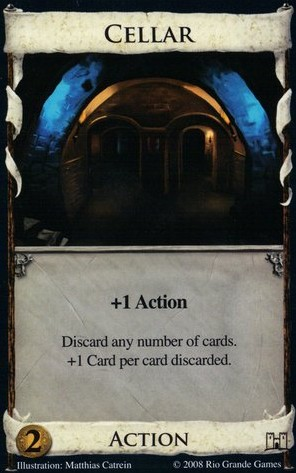
\includegraphics[width=.4\columnwidth]{cellar.jpg} \end{center}
\end{columns}
\inputminted
[ frame=lines
, framesep=2mm
, fontsize=\fontsize{1mm}{1mm} %\tiny
, linenos
] {haskell}{ComplexEffects.hs}
\footnotetext[1]{\tiny card image \& content by D. X. Vaccarino}
\end{frame}



% Demonstration (question 7)

\begin{frame} \frametitle{Demonstration}
\end{frame}



% Implementation & run-time system services (questions 8,9)

\begin{frame} \frametitle{Run-time System}
% Haskell game-engine
\end{frame}



% Evaluation of EDSL (question 11)

\begin{frame} \frametitle{Evaluation}
\begin{itemize}
\item Ease of use to describe all existing dominion cards
\item Time to program the equivalent cards in other data Languages: XML, JSON, YAML
\item In next iteration, when able to express card effects
  \being{itemize}
  \item How english-like expressing difficult card effects is
  \item How complex the card effects can be
  \item How intuitive it is to do both at the same time
  \end{itemize}
\end{itemize}
\end{frame}


% Future work - tools & libraries (questions 10,12)

\begin{frame} \frametitle{Future - Tool Support}
\begin{itemize}
\begin{small}
\item Type-checker
\item Debugging information
%  \begin{itemize}
%  \item Line numbers
%  \item Common programming mistakes
%  \item Mis-spellings (e.g. `Did you mean ...?`)
%  \end{itemize}
\item Automated card \emph{balancer} (e.g. `Maybe card XXX should be \$1 cheaper.`)
\item Develop more complex card examples for reference use
\item Library of AI players using various heuristics
\item Markup language conversion tools / support
\item Graphical (in-browser flash game?) client-server support
\end{small}
\end{itemize}
  \begin{center}
    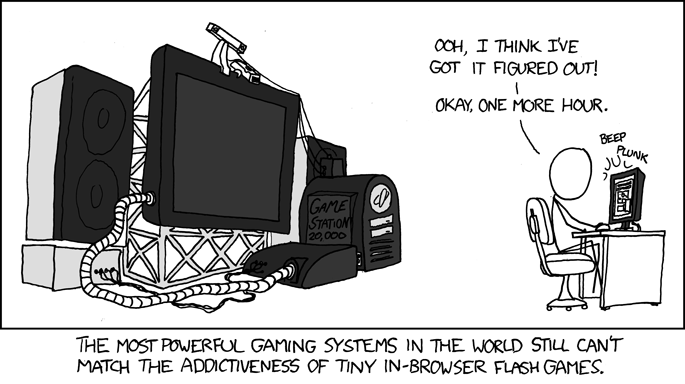
\includegraphics[width=.5\columnwidth]{flash_games.png}
  \end{center}
\end{frame}

\begin{frame} \frametitle{Future - Language Goals}
\begin{itemize}
\item Language support for English-like effect descriptions
\item Card-balancing algorithm
\item Comma-delimited syntactic sugar
\end{itemize}
\end{frame}



% Conclusion:

\begin{frame} \frametitle{Questions?}
Acknowledgements:
\begin{itemize}
\item Kathleen for Haskell and Language expertise
\item \href{http://learnyouahaskell.com/}{learnyouahaskell.com}
\end{itemize}
\begin{center}
  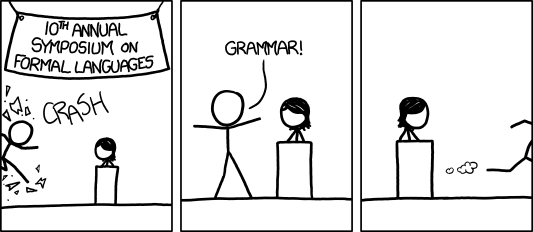
\includegraphics[width=.75\columnwidth]{formal_languages.png} \\
  {\tiny {[} audience looks around {]} 'What just happened?'
         'There must be some context we're missing.'}
\end{center}
\footnotetext[1]{
  {\tiny image from \href{https://xkcd.com/1090/}{xkcd.com/1090}}
}
\end{frame}



\end{document}
